\documentclass{article}
\usepackage[margin=1in]{geometry}
\usepackage{amsmath}
\usepackage{listings}
\usepackage{graphicx}
\usepackage{hyperref}
\usepackage[table]{xcolor} % For coloring tables
\usepackage{array} % For custom column widths
\usepackage{calc} % For calculating widths
\usepackage{float}

\graphicspath{ {./images/} }
\setlength{\parindent}{0pt}

\title{Using Minimax Algorithm to Make Connect 4 AI Agent}
\author{
\begin{tabular}{rl}
    Abdullah Elsayed Ahmed & 7459\\
    Mohammad Ashraf Hamdy & 7508\\
    Samah Abdelaziz Draz & 7889
\end{tabular}    
}

\date{March 20, 2024}

\begin{document}
\maketitle
\tableofcontents

\section{Introduction}
This is a basic connect4 game the player with more connected stack (Columns, Rows, Diagonals) will win the game.
We used Optimized AI agent to play against human so that the AI agent will win most of the time.
\begin{figure}[H]
    \centering
    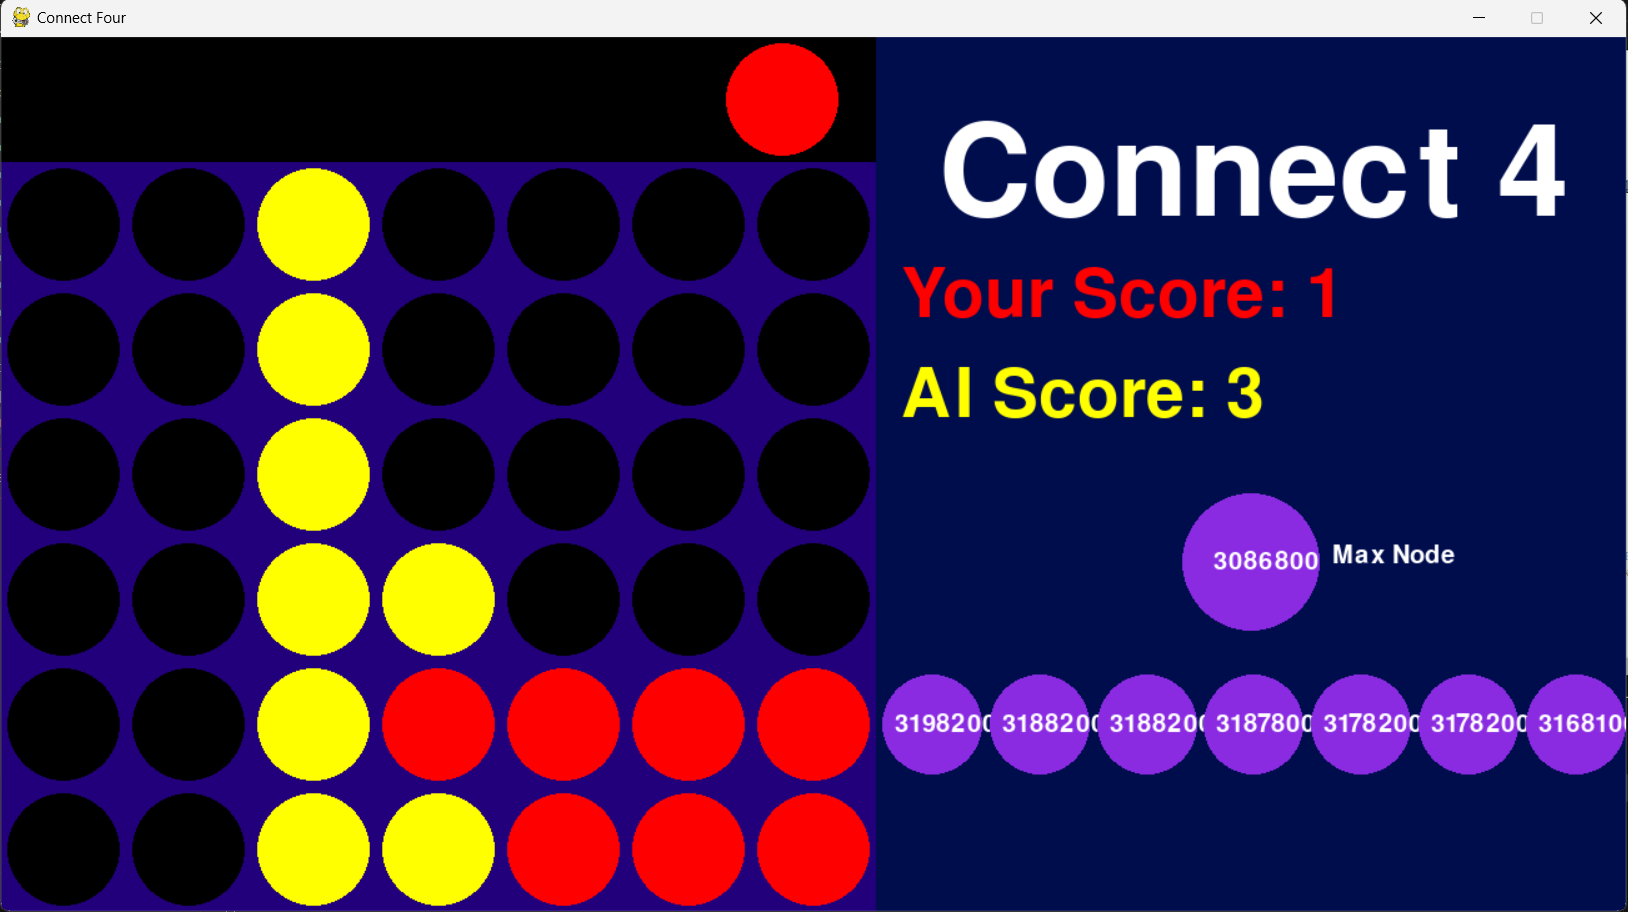
\includegraphics[width=0.8\linewidth]{GUI.png}
    \caption{Connect4 game GUI}
\end{figure}
\section{Game rules}
\subsection*{Board size}
Board size can be an where above or equal 7 in width and 6 in height.  
\subsection*{Evaluation} 
Each player has it own score based on number of 4 connected piece in the same row, column and diagonals the more connected 4 gain more score.

Example: 1,1,1,1,1,1,1. will be considered as \textbf{3 points} for player 1.

The player with higher score win the game.
\subsection*{Valid move}
The player can choose any column in the board but, It only legal if and only if the column isn't full.
\subsection*{Termination} 
Game terminate if and only if there is no more available spaces.

\section{GUI}
We made a sample user interface for the game using \textbf{pygame}, which enable the human to select the column by
hovering above it and click with the mouse to drop the piece and after short time the AI response and the game goes on until the board if full.

The GUI also show the score for Ai agent and human and also corresponding minimax trees for each move. 


\section{AI agent}
From mentioned rules We build our AI agent to fit those rules and try to get the max score to win.
\subsection*{Algorithm}
We used Minimax as our main algorithm, It is an decision-making algorithm, It have been used in our code to play against human in Connect4 game.
but We faced many challenges due to the full game tree is very huge $O(10^{35})$ so, We cuts the minimax tree at deeps K chosen before the game start.

We used different minimax algorithm
\begin{itemize}
    \item Normal minimax.
    \item Pruning minimax.
    \item Expectation minimax.
\end{itemize}
and We will talk about the different between them latter in the report.

\subsection*{Scoring}
Because We cut the minimax tree before termination state, We can't know the final score so, 
We had to choose a suitable heuristic algorithm to return a reasonable score.

A reasonable score tend to be high score if our AI agent will gain more points from a move and lower score from another move.

So our scoring will be based on the following:
\subsubsection*{Number of connected piece}[H]
We give the AI agent more score for the move which will have more consecutive pieces.
\begin{itemize}
    \item 4 connected: 1,000,000
    \item 3 connected: 40,000
    \item 2 connected: 10,000
\end{itemize}
\subsubsection*{Weighted center}
The player with more pieces at the center will a high change of winning so, We make a 2D matrix
which return higher score for the player with more pieces at the middle and less farther away.
\begin{center}
    \setlength{\tabcolsep}{2pt} % Adjust cell padding
    \renewcommand{\arraystretch}{1.5} % Adjust row height
    \begin{tabular*}{0.3217\textwidth}{|c|c|c|c|c|c|c|}
        \hline  
        \cellcolor{blue!25}300 & \cellcolor{blue!25}400 & \cellcolor{blue!25}500 & \cellcolor{green!25}700 & \cellcolor{blue!25}500 & \cellcolor{blue!25}400 & \cellcolor{blue!25}300 \\
        \hline  
        \cellcolor{blue!25}400 & \cellcolor{blue!25}600 & \cellcolor{green!25}800 & \cellcolor{green!35}1000 & \cellcolor{green!25}800 & \cellcolor{blue!25}600 & \cellcolor{blue!25}400 \\  
        \hline  
        \cellcolor{blue!25}500 & \cellcolor{green!25}800 & \cellcolor{green!35}1100 & \cellcolor{green!40}1300 & \cellcolor{green!35}1100 & \cellcolor{green!25}800 & \cellcolor{blue!25}500 \\  
        \hline  
        \cellcolor{blue!25}500 & \cellcolor{green!25}800 & \cellcolor{green!35}1100 & \cellcolor{green!40}1300 & \cellcolor{green!35}1100 & \cellcolor{green!25}800 & \cellcolor{blue!25}500 \\  
        \hline  
        \cellcolor{blue!25}400 & \cellcolor{blue!25}600 & \cellcolor{green!25}800 & \cellcolor{green!35}1000 & \cellcolor{green!25}800 & \cellcolor{blue!25}600 & \cellcolor{blue!25}400 \\  
        \hline  
        \cellcolor{blue!25}300 & \cellcolor{blue!25}400 & \cellcolor{blue!25}500 & \cellcolor{green!25}700 & \cellcolor{blue!25}500 & \cellcolor{blue!25}400 & \cellcolor{blue!25}300 \\  
        \hline  
    \end{tabular*}
\end{center}

\subsection*{Data structure}
We used \textbf{2D array} to represent our game board and used \textbf{hash table} to store previous board scores.  

\section{Results}
those are the result of our code each run shows the game board and corresponding minimax trees.
\subsection*{at k = 1}
\subsubsection*{Normal minimax}
\begin{center}
    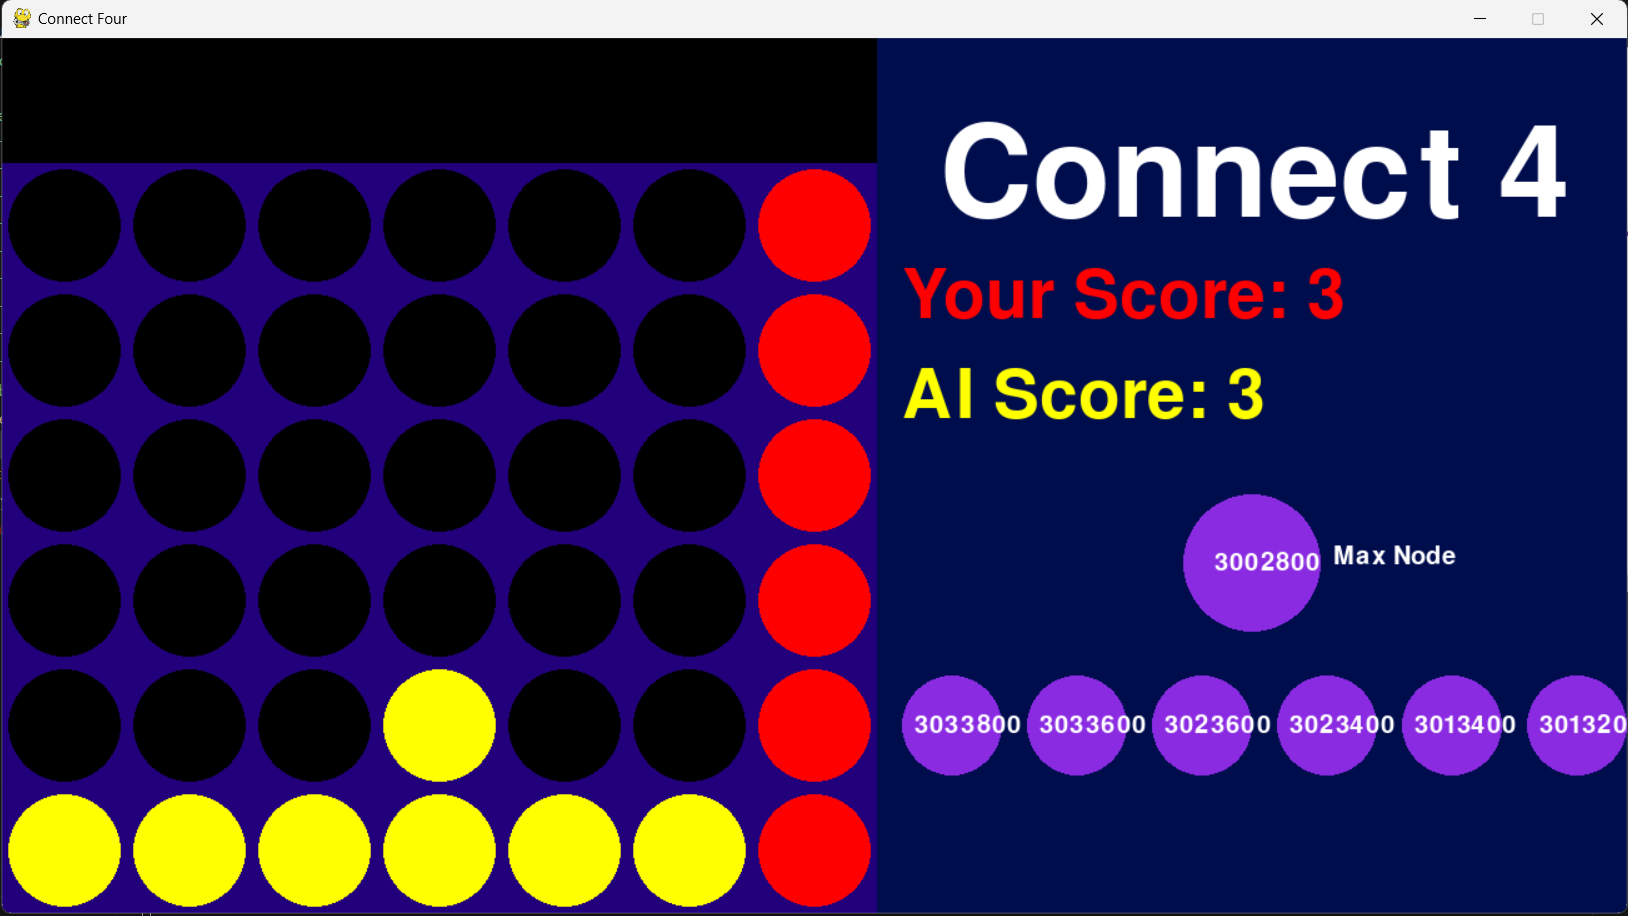
\includegraphics[width=0.8\linewidth]{testcase.png}
\end{center}
\begin{itemize}
    \item Nodes: 48
    \item Time: 0.004051923751831055
\end{itemize}
\subsubsection*{Pruning minimax}
\begin{center}
    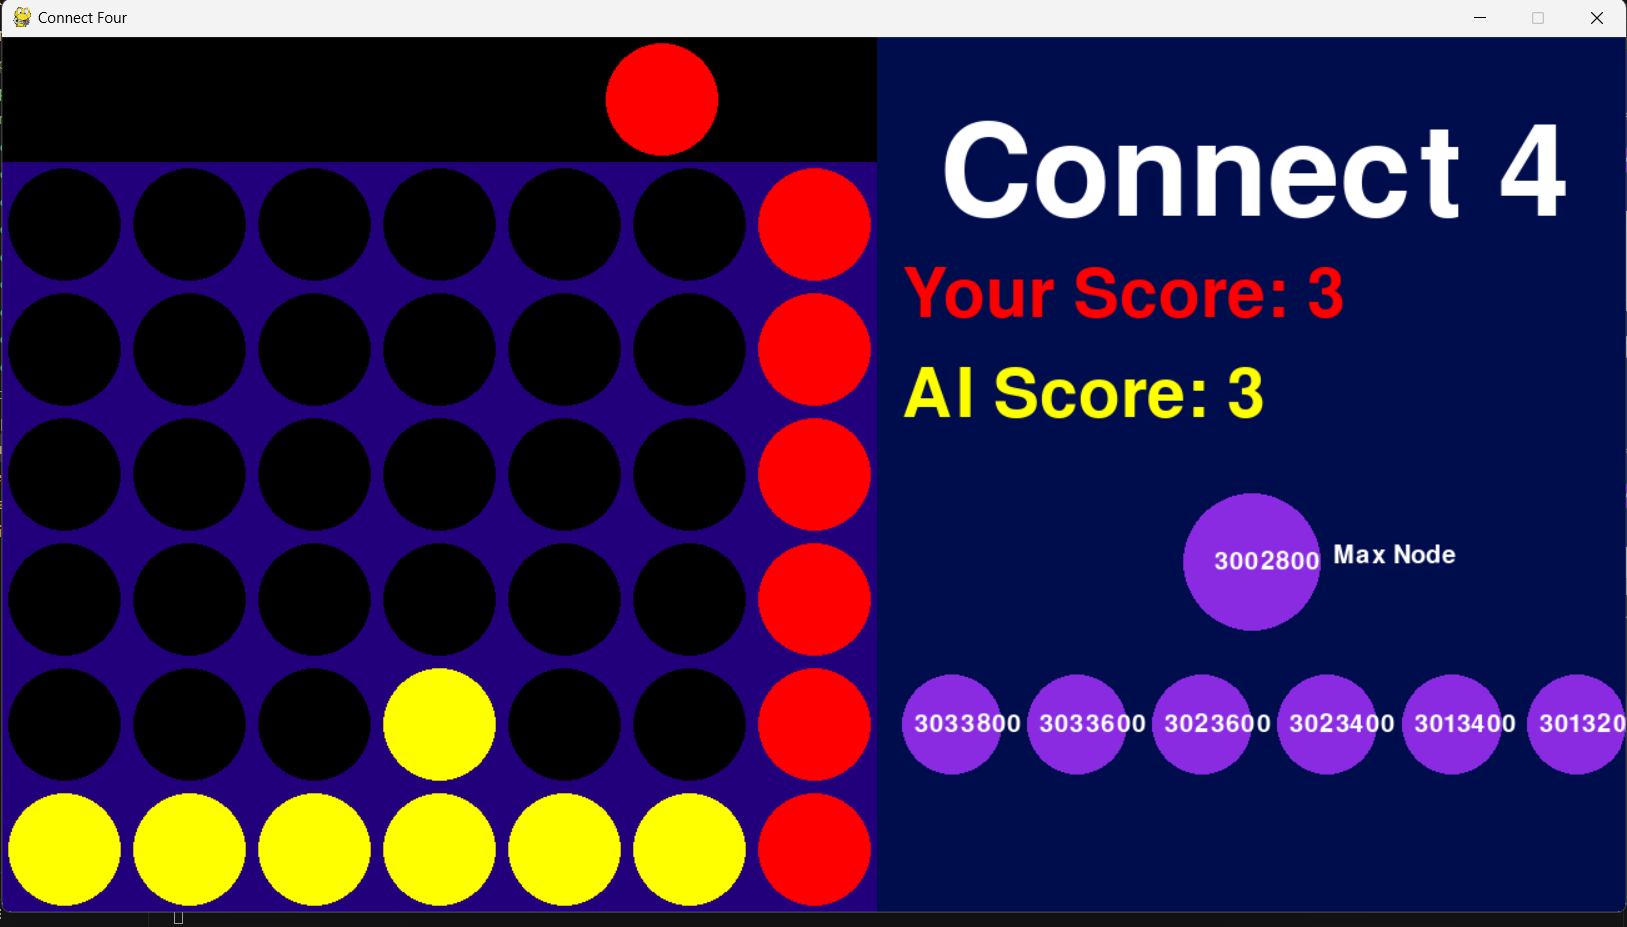
\includegraphics[width=0.8\linewidth]{pruning1.png}
\end{center}
\begin{itemize}
    \item Nodes: 48
    \item Time: 0.0041010379791259766
\end{itemize}
\subsubsection*{Expectation minimax}
\begin{center}
    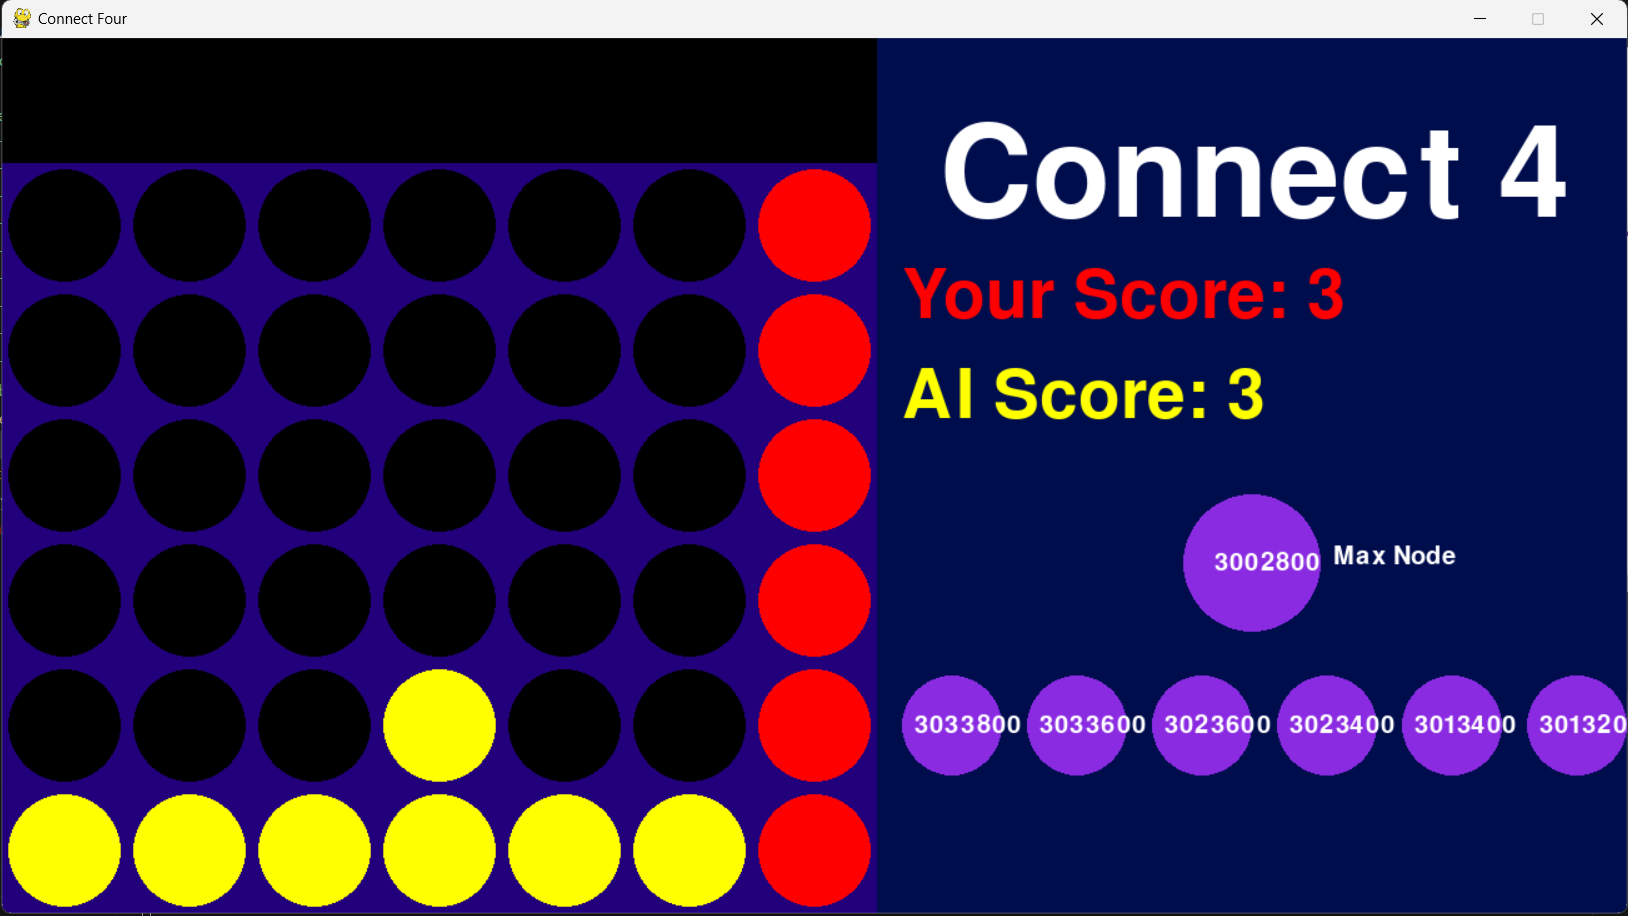
\includegraphics[width=0.8\linewidth]{testcase.png}
\end{center}
\begin{itemize}
    \item Nodes: 48
    \item Time: 0.004051923751831055
\end{itemize}
\subsection*{at k = 3}
\subsubsection*{Normal minimax}
\begin{center}
    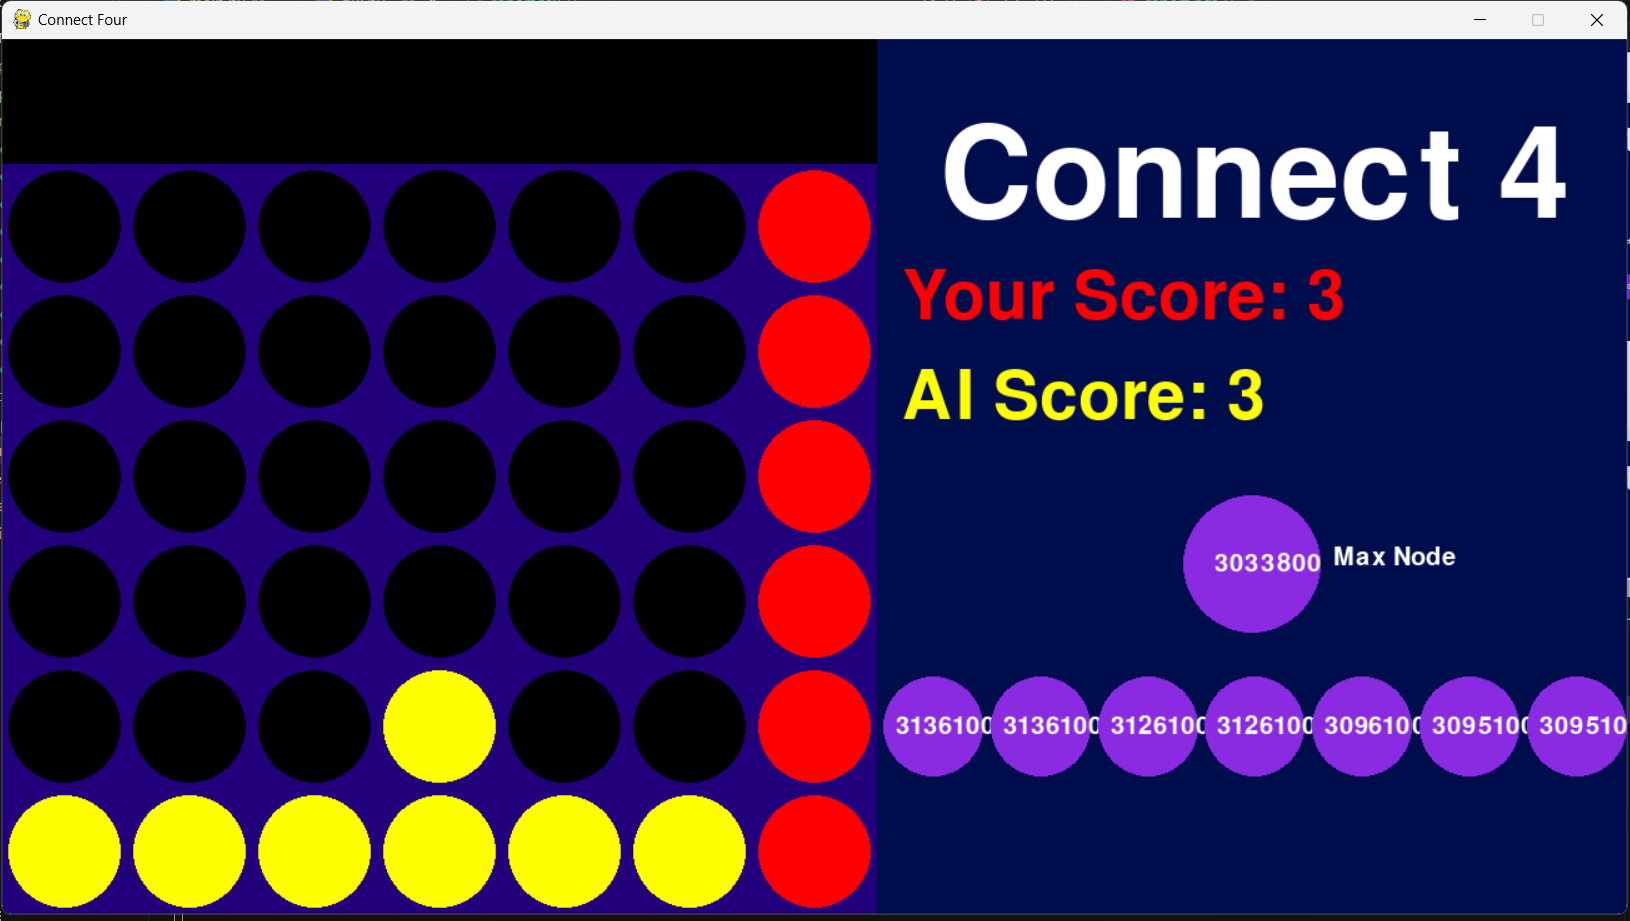
\includegraphics[width=0.8\linewidth]{testcase3.png}
\end{center}
\begin{itemize}
    \item Nodes: 2631
    \item Time: 0.12168431282043457
\end{itemize}
\subsubsection*{Pruning minimax}
\begin{center}
    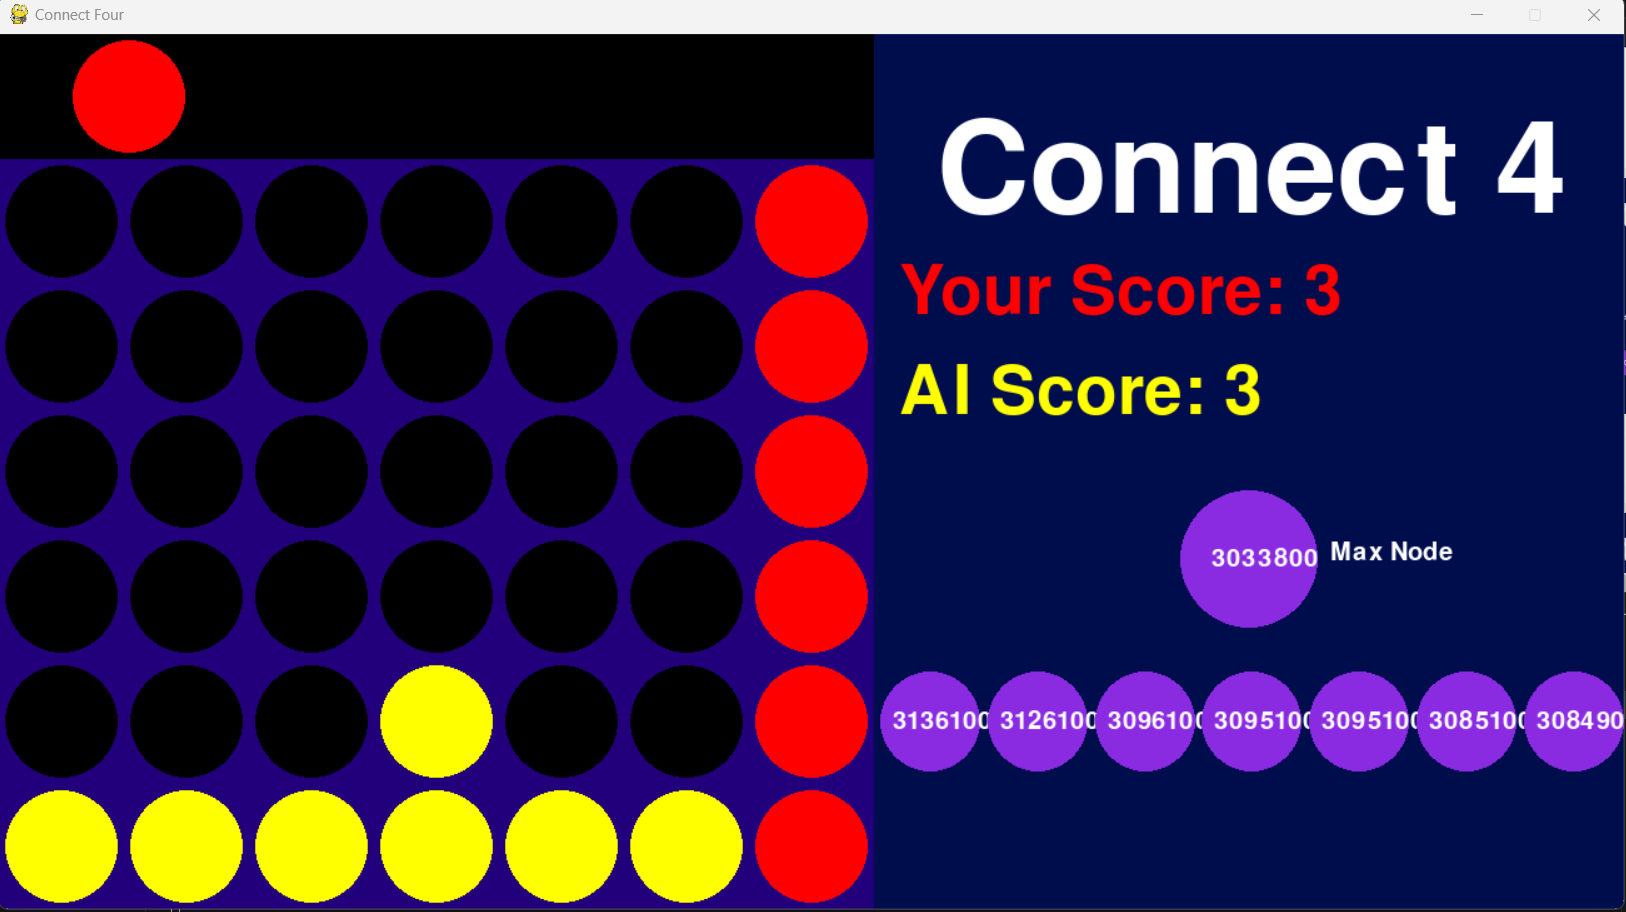
\includegraphics[width=0.8\linewidth]{pruning3.png}
\end{center}
\begin{itemize}
    \item Nodes: 1056
    \item Time: 0.04659581184387207
\end{itemize}
\subsubsection*{Expectation minimax}
\begin{center}
    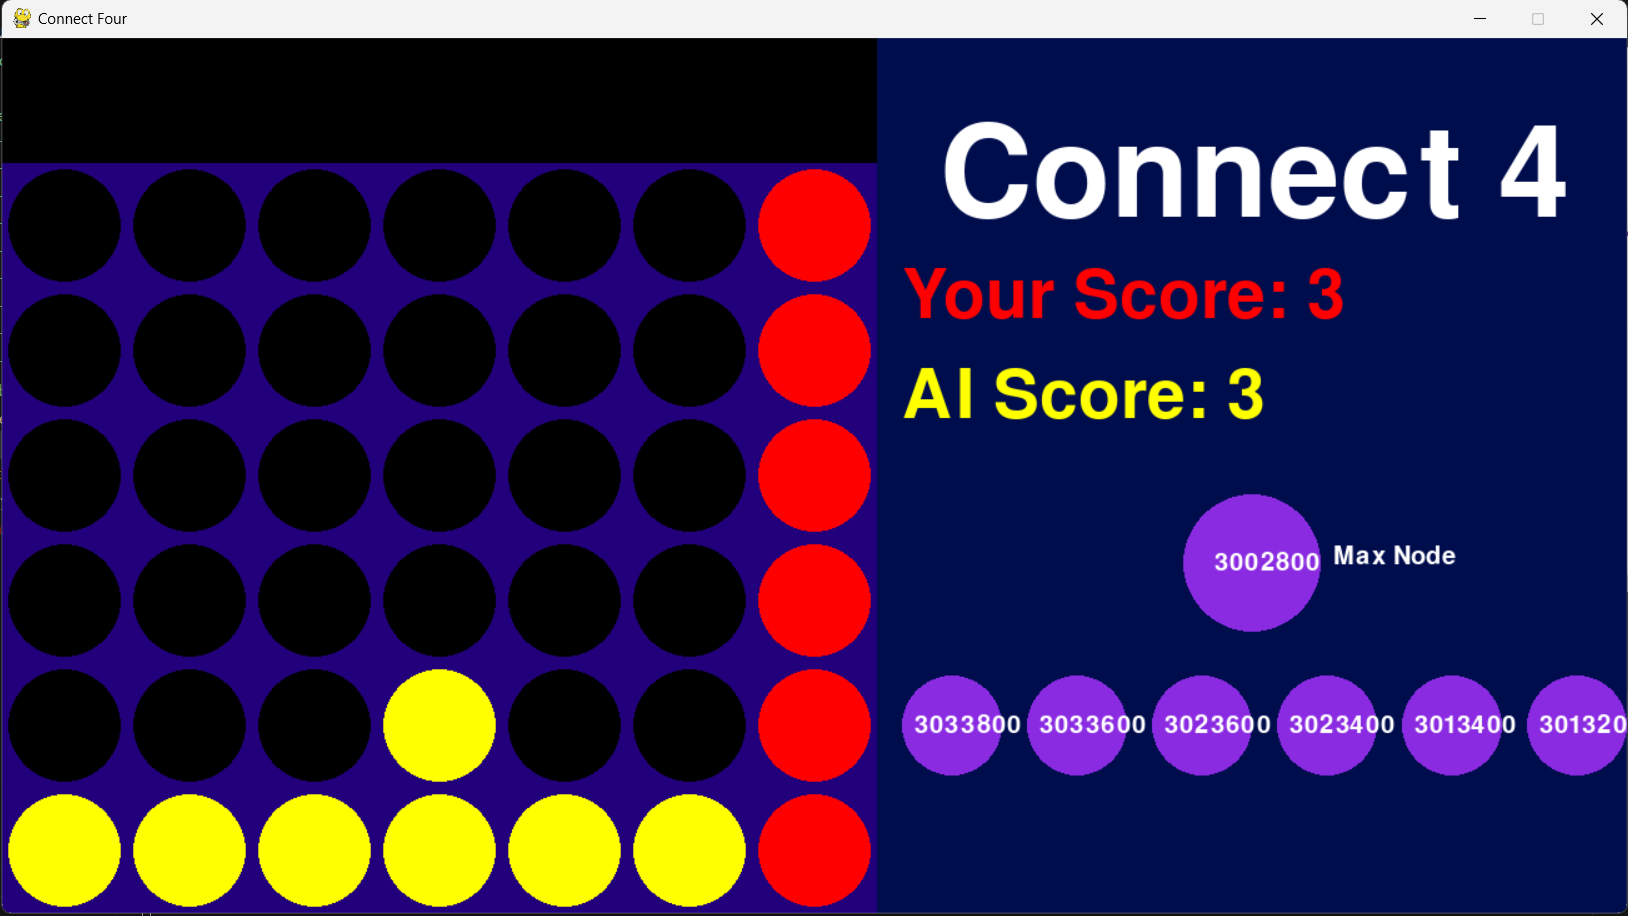
\includegraphics[width=0.8\linewidth]{testcase.png}
\end{center}
\begin{itemize}
    \item Nodes: 1056
    \item Time: 0.04659581184387207
\end{itemize}
\subsection*{at k = 5}
\subsubsection*{Normal minimax}
\begin{center}
    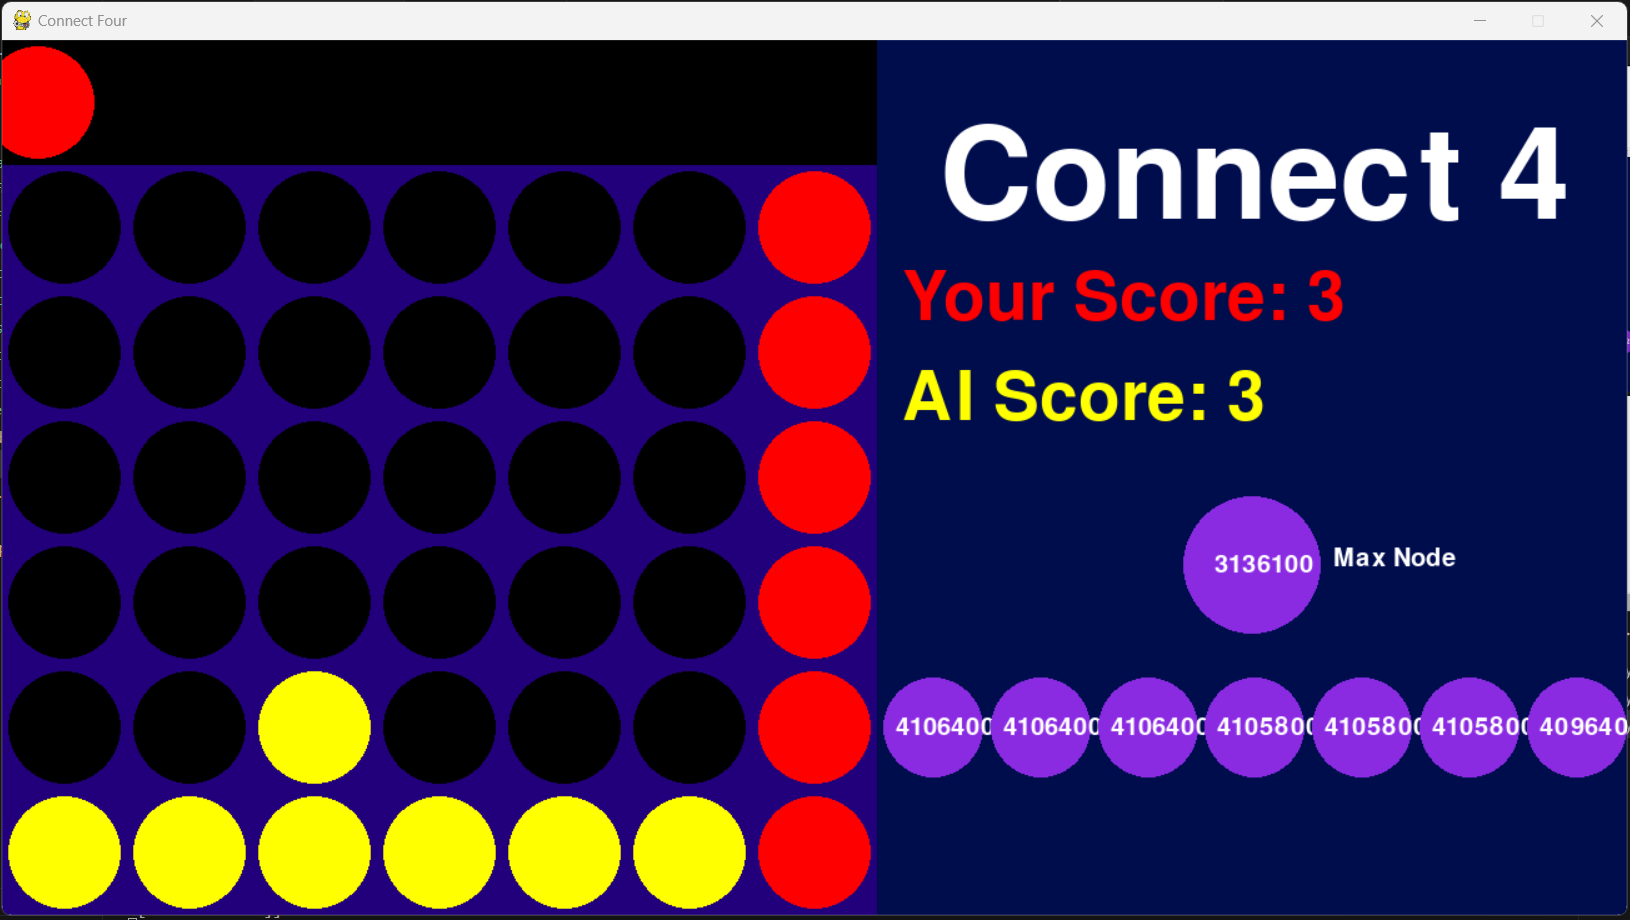
\includegraphics[width=0.8\linewidth]{testcase5.png}
\end{center}
\begin{itemize}
    \item Nodes: 62621
    \item Time: 1.756775140762329
\end{itemize}
\subsubsection*{Pruning minimax}
\begin{center}
    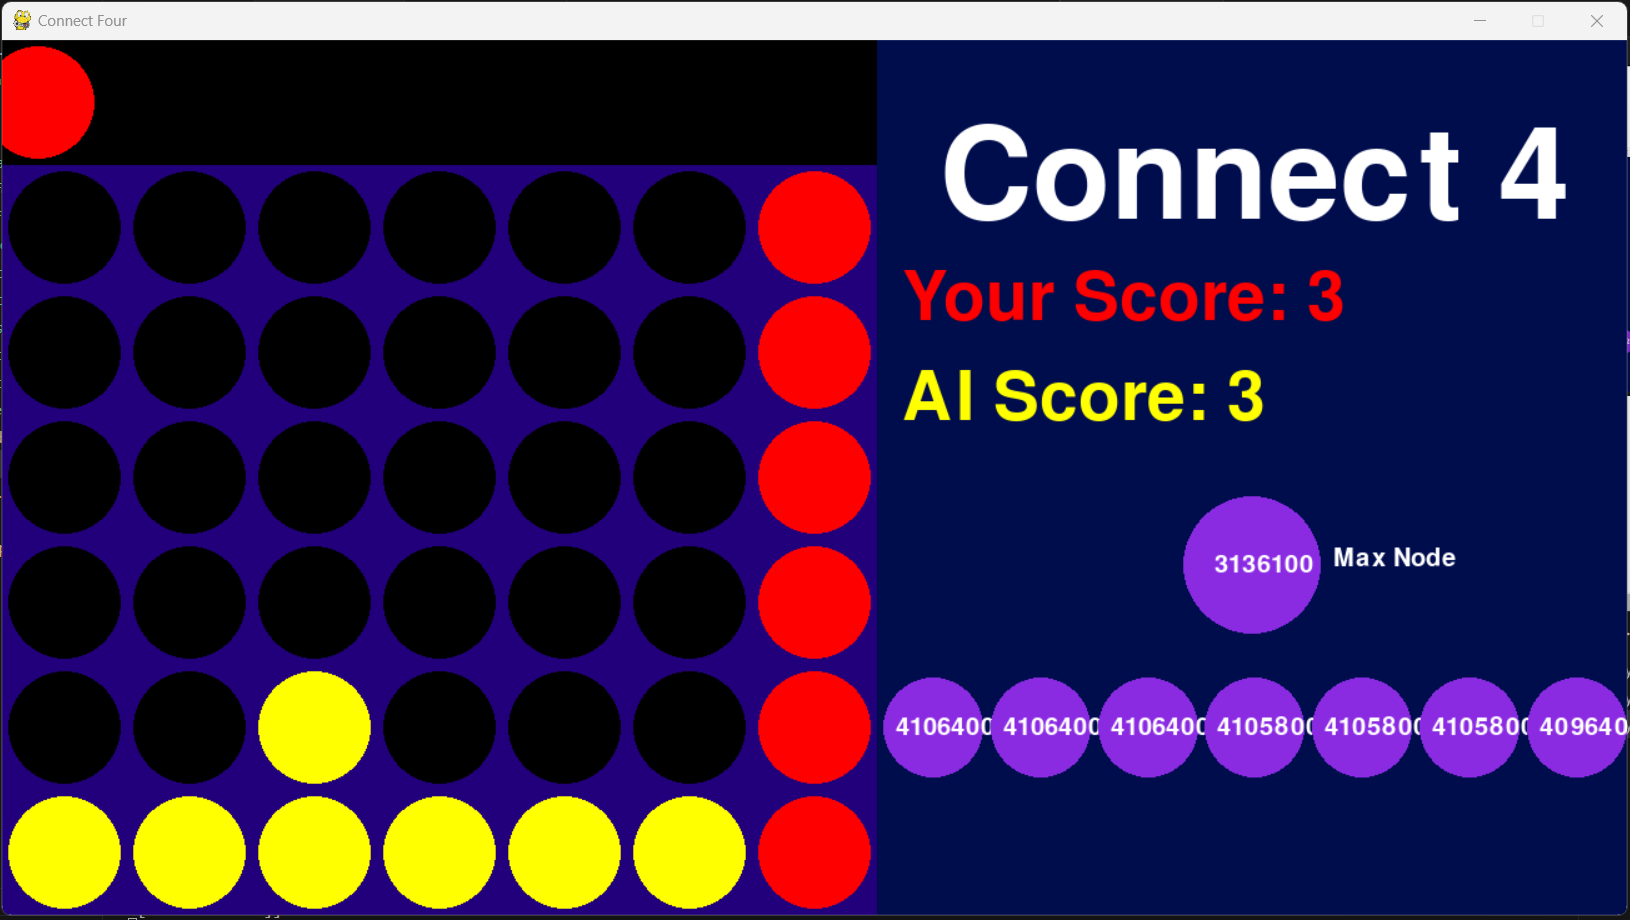
\includegraphics[width=0.8\linewidth]{pruning4.png}
\end{center}
\begin{itemize}
    \item Nodes: 11710
    \item Time: 0.6393032073974609
\end{itemize}
\subsubsection*{Expectation minimax}
\begin{center}
    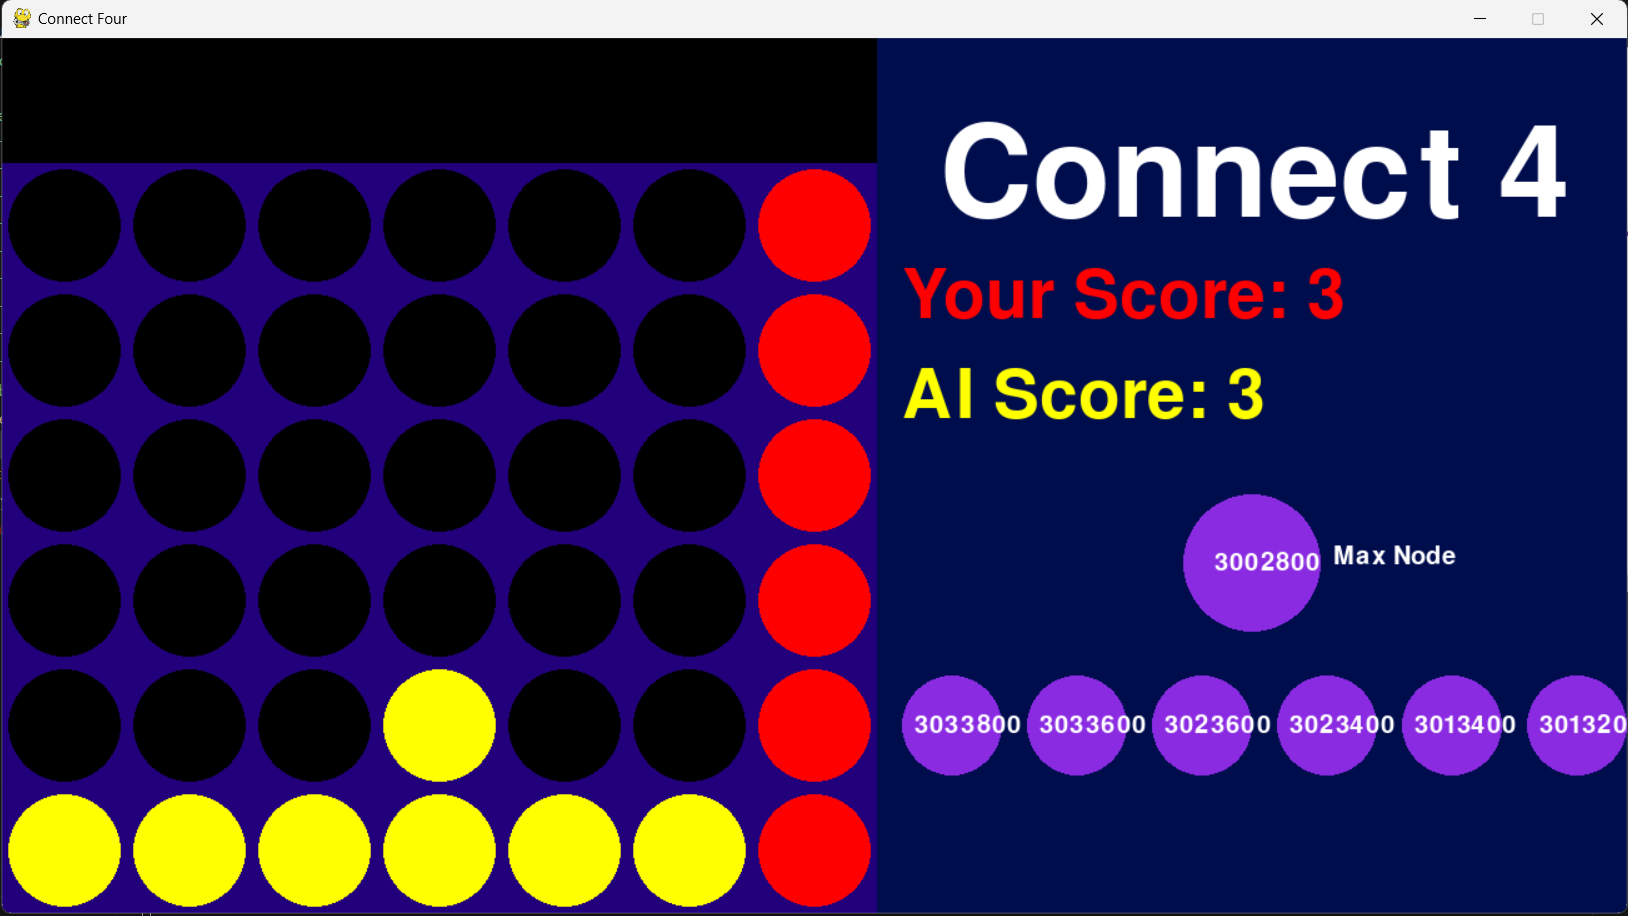
\includegraphics[width=0.8\linewidth]{testcase.png}
\end{center}
\begin{itemize}
    \item Nodes: 11710
    \item Time: 0.6393032073974609
\end{itemize}

\section{Conclusion}
From our result we can compare different minimax approach at different K values.

% \subsection*{at K = 1}
% \subsubsection*{Normal minimax}
% \subsubsection*{Pruning minimax}
% \subsubsection*{Expectation minimax}
% \subsection*{at K = 3}
% \subsubsection*{Normal minimax}
% \subsubsection*{Pruning minimax}
% \subsubsection*{Expectation minimax}
% \subsection*{at K = 5}
% \subsubsection*{Normal minimax}
% \subsubsection*{Pruning minimax}
% \subsubsection*{Expectation minimax}
\subsection*{In General}
\subsubsection*{Normal minimax}
It is the worst of them because It has to check losing move also it is not important no more (due to a better move is available).
\subsubsection*{Pruning minimax}
It is better version of normal minimax (minimax without alpha beta Pruning) due to the pruning process.
\subsubsection*{Expectation minimax}
It is slightly better then Pruning minimax.

\end{document}